\documentclass{article}
\usepackage[utf8]{inputenc}
\usepackage{blindtext}
\usepackage{tikz}
\usepackage{MnSymbol}
\usepackage{circuitikz}
\usepackage{cancel}
\usepackage{graphicx}
\graphicspath{ {images/} }
\usepackage{amsmath} % Required for \varPsi below
\usetikzlibrary{decorations.pathreplacing}
\usetikzlibrary{arrows}
\usepackage[export]{adjustbox}
\usepackage{enumitem}% http://ctan.org/pkg/enumitem
% https://tex.stackexchange.com/questions/78842/nested-enumeration-numbering

\begin{document}
\begin{titlepage}

ET Script


\end{titlepage}

\section{Übersicht}
\begin{enumerate}
  \item Defintion Ladung, Strom, Spannung, Potential
  \item Grundstromrkeis, Darstellung
  \item Widerstand $\Omega$ Ohmisches Gesetz
  \item Mehrteilige Schaltungen
  \begin{enumerate}[label*=\arabic*.]
    \item Stromknoten
    \item Spannungsmasche
    \item Superpostionsprinzip
  \end{enumerate}
  \item Reale Spannungs und Stromquellen
  \item Leistung
  \item Zeit abhänige Spannugen und Ströme
  \item Blindelement $L,C$
\end{enumerate}


\section{Elektronen}

Elektronische Ladung $Q$ besteht aus \underline{Elektronnen}\\
Stets \underline{negative} Ladung \\
(Postive Ladung ist Elektronenmangel, setzt Stoff vorraus)\\
1 Elektron hat eine Elementarladung von $e = 1,6 \cdot 10^{-19} A \cdot s$\\
\\
\\
$ Q = A \cdot s $ ($A/s$  Amper Sekunde) wegen negative: $q = -1,6 \cdot 10^{-19} A \cdot s$\\
\\
$Q_{Elektron} = -1,6 \cdot 10^{-19} A \cdot s$\\
Für úberschus\\
\\
\\
Eine Wolke hat eine Ladung von $Q_{wolke} = 1 As$\\
\\
$ Q = n * q$\\
$n$ ist die Anzahl der $E$\\
$n = ? $\\
\\
$n = \frac{Q}{q} = \frac{1 As}{-1,6 \cdot 10^{-19} As}$\\
\\
Wir können kürzen:\\
$\frac{1 \cancel{As}}{-1,6 \cdot 10^{-19} \cancel{As}}$\\
$\approx \frac{1}{-1,6} \cdot 10^{19}$\\
$\approx \frac{5}{8} \cdot 10^{19}$\\
\\

\section{Spannung}
\underline{Spannung ist ein Zustand}\\
platzhalter bild\\
Es herrscht eine \underline{Spannung $U$}\\
Oder Wolke 2\\
Platzhalter bild2\\
$ U > 0 $\\
\\

Wolke3\\
Platzhalter Bild3\\

Spannungsrichtung festlegung mit einem Zählpfeile (\underline{willkührliche Annahme})\\
hier Spannung von Erde zur Wolke \underline{positive}\\
\\
Einheit der Spannung\\
Volt, kurz $V$\\
\\
Angabe ziB $U = + 230 V \leftarrow $ Buchstabe als Einheit\\

\newpage

Vorsätze

$ 1 =1 $\\
$ 1000 = 10^3 = k $ (kilo)\\
Übersicht:\\
$ 10^{-12} = p $ ("pico")\\
$ 10^{-9} = n $ ("nano")\\
$ 10^{-6} = \mu $ ("mikro")\\
$ 10^{-3} = m $ ("milli")\\
$ 10^{-2} = c $ ("centi")\\
$ 10^{-1} = d $ ("deci")\\
$ 10^{1} = da $ ("deca")\\
$ 10^{2} = h $ ("hecto")\\
$ 10^{3} = k $ ("kilo")\\
$ 10^{6} = M $ ("mega")\\
$ 10^{9} = G $ ("giga")\\
$ 10^{12} = T $ ("tera")\\


\section{Strom}

\underline{Strom} ist die Bewegung von Elektronen. (d.h "Ladung fließt")

Gleichstrom, Konstanter Elektronenfluß.


\begin{figure}[h]
  \begin{center}
   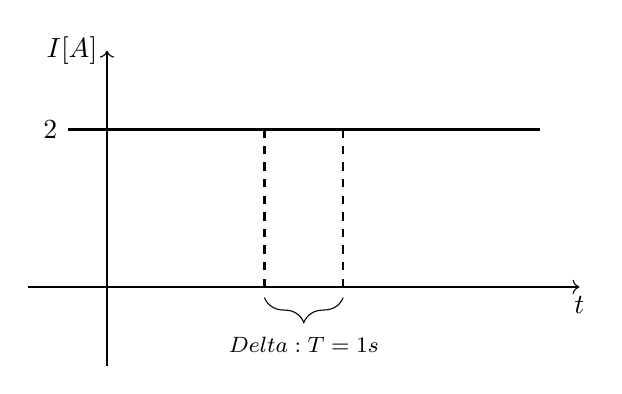
\begin{tikzpicture}
    \draw[->] (0,-1) -- (0,3) node[anchor=east] {$I [A]$};
    \draw[->] (-1,0) -- (6,0) node[anchor=north] {$t$};
    \draw[thick] (-0.5,2) node[anchor=east] {$2$}-- (5.5,2) ;
    \draw[thick,dashed] (2,0) -- (2,2);
    \draw[thick,dashed] (3,0) -- (3,2);
    \draw [decorate,decoration={mirror,brace,amplitude=9pt},yshift=-1pt](2,-0.1) -- (3,-0.1) node [black,midway,yshift=-0.6cm] {\footnotesize $Delta: T=1s$} ;
   \end{tikzpicture}
  \end{center}
\end{figure}

Aussage: Gleichstrom: $I = 2 \cdot A$\\
Zeit als ein interval\\
Zeit in Allgemeinen als Zeitabschnitt Benutzt, dann $T$\\
\\
Definition:\\
Strom $I$ ist fliesende Ladung $Q$ pro Zeit intervall $T$ damit $ I[A] = \frac{Q[A\cdot s]}{T[s]} $\\
Bespiel ergäbe:\\
$ Q = I \cdot T$\\
Wie = $2 A \cdot 1s  = \underline{2 As} $\\
Üblich: Kurzes Zeit intervall $\Delta T$\\
\\
$ I = \frac{\Delta Q}{\Delta T} \rightarrow \frac{d Q}{d t} $  
$ lim \Delta \rightarrow 0 $ \\
\\
Beschreiben von Strömlichen veränderung (nicht gleich Strom) diese Gleichung gilt auch für Zeit veränderliche Ströme.\\
\\
(Ableitung der Steigung nder der Zeit = Anstieg).\\



\section{Zeit abhänige Ströme und Spannungen}

Zeit eigentlich Kontunierlich und ständig ablaufend.
\underline{Gleichstrom} und \underline{Gleichspannung} sind streng genommen Einbildung, müssten ewig daueren

In der Realität geht es immer um Zeitinvervalle. \newline

\begin{tikzpicture}

% horizontal axis
\draw[->] (0,0) -- (6,0) node[anchor=north] {$t$};
% ranges

% T1 line
\draw[dotted] (2,0) -- (2,3);
\draw	(2.3,2.5) node{{$t_1$}};

%T2 Line
\draw[dotted] (4,0) -- (4,3);
\draw	(4.3,2.5) node{{$t_2$}};

% Our BLock
\draw[thick] (2,0) -- (2,2) -- (4,2) -- (4,0);
\draw (1,1) node {$10 V$}; %label

% Strom
\draw[thick,dashed] (0,2) -- (6,2);
\draw (5,1.8) node {\scriptsize Gleichstrom}; %label

\end{tikzpicture}
\newline
!Üblicher Sprachgebrauch "Gleichspannungs"

aber wenn $t_2 - t_1 = T$

Zeitintervall Implusdauer
Gewisse Willküre
insbesondere Wahl Zeitpunkt Null ist praktisch, aber oft beliebig


In betrachteten Zeitintervall sind auch beliebige Verläufe als Gleichwert möglich
Extremfall: Rauschen stochastisches Verhalten ohne Regelmässigkeit
Auch im betrachten Zeitintervall kann es Widerholungen geben

Üblich beiu sich wiederholende Vorgängen: Periodendauer $T_0$

Beispiel:
\newline

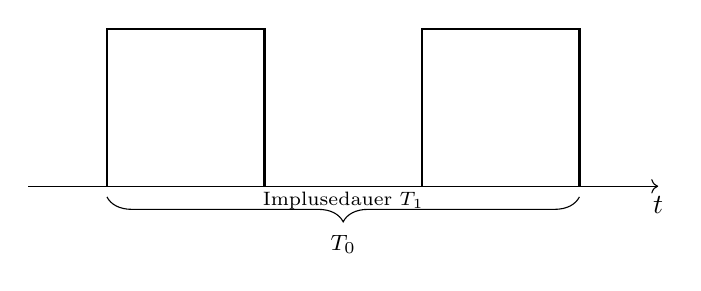
\begin{tikzpicture}

% horizontal axis
\draw[->] (0,0) -- (8,0) node[anchor=north] {$t$};
% ranges

% Our BLock
\draw[thick] (1,0) -- (1,2) -- (3,2) -- (3,0);

\draw[thick] (5,0) -- (5,2) -- (7,2) -- (7,0);
\draw [decorate,decoration={mirror,brace,amplitude=9pt},yshift=-1pt](1,-0.1) -- (7,-0.1) node [black,midway,yshift=-0.6cm] {\footnotesize $T_0$}node[midway,yshift=-0.05cm] {\scriptsize Implusedauer $T_1$};

\end{tikzpicture}

\begin{tikzpicture}

% horizontal axis
\draw[->] (0,0) -- (8,0) node[anchor=north] {$t$} node [yshift=0.6cm]{\scriptsize Sinus Funktion};
% ranges

% Our BLock
\draw[thick] (0,0) sin (2,2) cos (4,0) sin (6,-2) cos (8,0) ;

\end{tikzpicture}

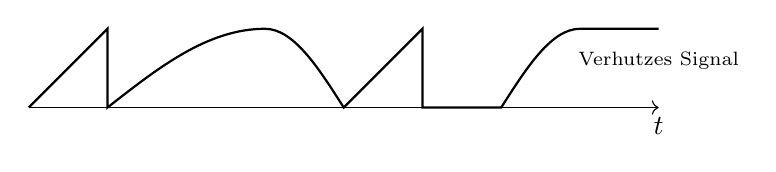
\begin{tikzpicture}

% horizontal axis
\draw[->] (0,0) -- (8,0) node[anchor=north] {$t$} node [yshift=0.6cm]{\scriptsize Verhutzes Signal};
% ranges

% Our BLock
\draw[thick] (0,0) -- (1,1) -- (1,0) sin (3,1) cos (4,0) -- (5,1) -- (5,0) -- (6,0) sin (7,1) -- (8,1);

\end{tikzpicture}

Bei zeit abhaenigen Spannungen und Strömen kommen die Elemnte Kondensator und Induktivität, bei welcher der Spannungs-Strom verhalten nicht mehr durch das ohmische Gesetz beschrieben werden kann, zur Geltung.
(Also: Spannung und Strom beim Kondensator und der Induktivität haben nicht den gleichen Zeit verlauf)


\subsection{Schaltzeichen}


\begin{figure}[h!]
  \begin{center}
    \begin{circuitikz}
    \draw (0,0) to[C=$C_1$] (0,1);
    \draw (4.5,0.5) node {Kondesator ($\hat{=}$ Kapazität $C$, Einheit "Farad")};
    \end{circuitikz}
  \end{center}
\end{figure}

\begin{figure}[h!]
  \begin{center}
    \begin{circuitikz}
    \draw (0,0) to[L=$L_1$] (0,1);
    \draw (4.5,0.5) node {Induktivität ($H$, Einheit "Henry")};
    \end{circuitikz}
    \newline
    \begin{circuitikz}[european]
        \draw (0,0) to[L=$L_1$] (0,1);
        \draw (4.5,0.5) node {z.b in Deutschland gelegentlich};
     \end{circuitikz}
  \end{center}
\end{figure}

\subsection{Kondensator}
Platten Kondensator:


\subsection{Wechselspannung und Wechselstrom}


\begin{figure}[h!]
  \begin{center}
\begin{tikzpicture}

% axis
\draw[->] (-1,0) -- (9,0) node[anchor=north] {$t$};
\draw[->] (0,-2) -- (0,2) node[anchor=east] {$u(t)$};
% ranges

% Our BLock
\draw[thick] (0,0) sin (2,2) cos (4,0) sin (6,-2) cos (8,0) ;

\end{tikzpicture}
  \end{center}
\end{figure}



Praktisch

Bei der Umwaldung von mechanischer Energie in elektronische Energie ist eine \underline Drehbewegung("Generator") besonders effektiv. Dabei entsteht eine Sinusförmiger Spannungsfrom. Die gesmate Energieversorung beruht drauf.


Allgemeine periodische Verlaüfe 

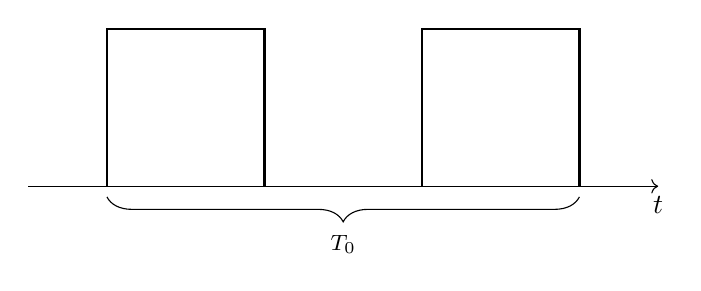
\begin{tikzpicture}

% horizontal axis
\draw[->] (0,0) -- (8,0) node[anchor=north] {$t$};
% ranges

% Our BLock
\draw[thick] (1,0) -- (1,2) -- (3,2) -- (3,0);

\draw[thick] (5,0) -- (5,2) -- (7,2) -- (7,0);
\draw [decorate,decoration={mirror,brace,amplitude=9pt},yshift=-1pt](1,-0.1) -- (7,-0.1) node [black,midway,yshift=-0.6cm] {\footnotesize $T_0$};

\end{tikzpicture}

Anzahl der periodischen Vorgänge im Messzeitintervall $T_M(T_M>>T_0)$ zählen umd damit die Häufigkeit ausdürcken. Andere Ausdürck für Häufigkeit: \underline{Frequenz} $f$ 

$f = \frac{1}{T_0}$ Einheit kann $S^{-1}$ sein besser \underline{$Hz$}.


Damit wird eine Sinusspannung darstellen mit:\newline
$u(t) = \hat{U} \cdot \sin(\varphi(t))$  



$ = \hat{U} \cdot \sin(\frac{t}{t_0} \cdot 360^{\circ})$ Deinition aus Frequenz $f$ und $2\pi$ wird die Winkelfrequenz \fbox{$\omega = 2\pi \cdot f$} \newline
$ = \hat{U} \cdot \sin(f \cdot t \cdot 360^{\circ}) $ Damit wird \fbox{$u(t) = \hat{U} \cdot \sin(\omega t)$} wichtigste Darstellung oder Kreisfrequenz.\newline
$ = \hat{U} \cdot \sin(f \cdot t \cdot 2\pi) $ Bogenmass Wenn der Startpunkt nicht bei Null liegt.
\begin{figure}[h!]
  \begin{center}
\begin{tikzpicture}

% axis
\draw[->] (-1,0) -- (9,0) node[anchor=north] {$t$};
\draw[->] (0,-2) -- (0,2) node[anchor=east] {$u(t)$};
\draw[->] (2,0) -- (2,1.9) node[anchor=south,yshift=1pt] {$\hat{U}$};
% ranges

% Our BLock
\draw[thick] (0,0) sin (2,2) cos (4,0) sin (6,-2) cos (8,0) ;

\end{tikzpicture}
  \end{center}
\end{figure}

$\Delta t$ ausdürckbar als Winkel $[ ^{\circ}]$, Bogenmass oder Zeitmass entspricht, Phasenverschiebung Eingentwinkel Winkel $\varphi \leadsto u(t)(\omega t + \varphi)$ \underline{Die Parameter}

Darstellung in der Schaltung als Symbol:
\begin{figure}[h!]
  \begin{center}
    \begin{circuitikz}[european]
        \draw (0,0) to[V] (0,1);
        \draw (4.5,0.5) node {$\hat{U} \sin(\omega t + \varphi)$};
     \end{circuitikz}
  \end{center}
\end{figure}

\newpage
Schaltung mit Sinusspannung und ohmischen Widerständen


es war $I = \frac{U}{R}$ $R$ fest, dann $I$  \texttt{\char`\~}  $U$
\begin{figure}[h!]
  \begin{center}
    \begin{circuitikz}[european]
      \draw (0,0)
      to[V,v=$U_q$] (0,2) % The voltage source
      to[short] (4,2)
      to[R=$R_1$] (4,0) % The resistor
      to[short] (0,0);
     \end{circuitikz}
  \end{center}
\end{figure}

Leistung

momentan: $u \cdot i$
Maximal $\hat{U} \cdot \hat{I}$

Mit $\hat{I} = \frac{\hat{U}}{R} \leadsto i(t)=\hat{I} \cdot \sin(\omega t) = \frac{\hat{U}}{R} \cos \sin(\omega t)$


$P(t) = \hat{U} \cdot \hat{I} \cdot [\sin(\omega t)]^{2} $

\begin{figure}[h!]
  \begin{center}
	\begin{tikzpicture}

	% axis
	\draw[->] (-1,0) -- (9,0) node[anchor=north] {$t$};
	\draw[->] (0,-2) -- (0,2) node[anchor=east] {$P(t)$};
	% ranges

	% Our BLock
	\draw[thick] (0,0) sin (2,2) cos (4,0) sin (6,2) cos (8,0) ;
	\draw (0,1.5) node[anchor=east]{$\frac{1}{2}\cdot\hat{U}\cdot\hat{I} $}[thick,dashed] (0,1.5) -- (8,1.5) ;

	\end{tikzpicture}
  \end{center}
\end{figure}

Dabei entsteht $2\omega$!(Frequenzverdopplung)

$[\sin(\omega t)]^2\cdot\frac{1}{2}[1-\cos(2 \omega t)] $

Die mittlere oder \underline{Effektive} Leistung ist \fbox{$\frac{\hat{U}\cdot\hat{I}}{2}=P_{eff}$} oder 
$ \frac{\hat{U}}{\sqrt{2}} \cdot \frac{\hat{I}}{\sqrt{2}}= \frac{\hat{U}\cdot\hat{O}}{2}$

Definition der effetiven Spannung
$U_{eff} = \frac{\hat{U}}{\sqrt{2}} $ oder $ \hat{U} = U_{eff} \cdot \sqrt{2} $

$U_{eff}$ = Netzspannungsangabe hier \underline{$230V$} und \underline{$f=50Hz$}

Alle Berechnungen mit Gleichspannug und Gleichströmen sind in Widerstandskreisen auf Wechselspannungen und -strömen übertragbar.

\newpage
\subsection{Sinusspannungen und Ströme bei $L$ und $C$}

\begin{figure}[h!]
  \begin{flushleft}
    \begin{circuitikz}
    \draw (0,0) to[C=$C$] (0,1);
    \end{circuitikz}
    \newline
    $ u(t) = \frac{1}{C} \int i(t) \cdot dt$ \newline
	$ C \cdot \frac{d u(t)}{dt} = i(t)$

  \end{flushleft}
\end{figure}

\begin{figure}[h!]
  \begin{center}
	\begin{tikzpicture}

	\draw[->] (-1,0) -- (9,0) node[anchor=north] {$t$};
	\draw[->] (0,-2) -- (0,2) node[anchor=east] {$u(t)$};
	\draw[thick] (0,0) sin (2,2) cos (4,0) sin (6,-2) cos (8,0) ;

	\end{tikzpicture}
	\begin{tikzpicture}

	\draw[->] (-1,0) -- (9,0) node[anchor=north] {$t$};
	\draw[->] (0,-2) -- (0,2) node[anchor=east] {$u(t)$};
	\draw[thick] (0,2) cos (2,0) sin (4,-2) cos (6,0) sin (8,2) ;

	\end{tikzpicture}
  \end{center}
\end{figure}

"Im Kondensator elit der Strom vor."



Das Konzept $ R = \frac{U}{I}$ war sehr praktisch. Problem hier?


extrme änderung öber die Zeit bzw. Periode
Problem ist die Verschiebung unzwecksmässiger Versuch


\subsection{Imaginäre Zahl $j$}


Der Strom durch den Kondensator hat eine - wenn auch zeitlich vershene - Sinusform. Phasenverschiebung $ 90^{\circ} \hat{=} \frac{\pi}{2} \hat{=} \frac{T_0}{2}$


\newpage

\section{Übertragungsvewrhalten von komplexen Schaltung bei sinförmiger Erregung} % (fold)


Grund: Vierpole

\begin{figure}[h]
    \centering
    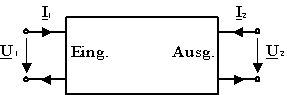
\includegraphics[width=0.65\textwidth,left]{dito01}
    \caption{Vierpole}
    \label{fig:1}
\end{figure}
\setlength{\parindent}{0cm} 


Zuordnung der Richtung per definition (üblich) \newline

Passive Vierpole (ohne Verstärker) haben stets eine kleinere Singalausgangsleistung als Eingangsleitung. Hier in ET1 Beschränkung auf passive Vierpole und nur Spannungsübertragung.


\begin{center}
Def:
 Spannungsverstärkung $v_u$ ist $v_u = \frac{u_2}{u_1}$
\end{center}

weitere Beschränkung Sinusspannung

Beispiel 1:

\begin{figure}[h]
  \begin{center}
    \begin{circuitikz}[european]
        \draw
        (0,0) to [short, o-] (2,0)
        to  (2,0)
        to[R, l=$R_1$] (3,0)
        to [short, -*] (4,0)
        to[R, l=$R_2$] (4,-2)
        to   (4,-2)
        (0,-2) to [short, o-*] (4,-2)
        (4,-2) to [short, -o] (7,-2)
        (4,0) to [short, -o](7,0);

        \draw[-latex] (0,-0.1) -- (0,-1.9);
     \end{circuitikz}
  \end{center}
\end{figure}
\newpage
Kann umgezeichnet werden:

Spannungsteiler
\begin{figure}[hb]
  \begin{center}
    \begin{circuitikz}[european]
        \draw
        (0,0) to [short, o-*] (2,0)
        to (2,-1)
        to[R, l=$R_1$] (2,-2)
        to (2,-3)
        to[R, l=$R_2$] (2,-4)
        to   (2,-5)
        (2,-2.5) to [short, *-o] (4,-2.5)
        (0,-5) to [short, o-*] (2,-5)
        (2,-5) to [short, -o](4,-5);

        \draw[-latex] (0,-0.1) -- (0,-4.9) node[midway,anchor=east]{$U_1$};
        \draw[-latex] (4,-2.6) -- (4,-4.9) node[midway,anchor=west]{$U_2$};
     \end{circuitikz}
  \end{center}
\end{figure}

hier sowohl Gleichspannug als $u(t) = \hat{U} \cdot \sin \omega t $ \newline
$ u_1 = \frac{R_1}{R_1 + R_2} \cdot u_2$ \newline
$ v_u = \underset{"Teilfaktor"}{\frac{Teilwiderstand}{Gesamtwiderstand}}  $ oder $ u_2 = \frac{R_2}{R_1 + R_2} \cdot u_1$ \newline
$\leadsto v_u = \frac{R_2}{R_1 + R_2} $ \\


Beispiel 2:

\begin{figure}[h!]
  \begin{center}
    \begin{circuitikz}[european]
        \draw
        (0,0) to [short, o-] (2,0)
        to  (2,0)
        to[R, l=$R_1$] (3,0)
        to [short, -*] (4,0)
        to[C, l=$C_1$] (4,-2)
        to   (4,-2)
        (0,-2) to [short, o-*] (4,-2)
        (4,-2) to [short, -o] (7,-2)
        (4,0) to [short, -o](7,0);

        \draw[-latex] (0,-0.1) -- (0,-1.9);
     \end{circuitikz}
  \end{center}
\end{figure}
Allegemeine Formal:

$ v_u(\omega) = \frac{\frac{1}{j\omega C}}{R_1 + \frac{1}{j\omega C}} $ \newline
$ v_u(\omega) = \frac{\frac{1}{j\omega C}}{R_1 + \frac{1}{j\omega C}} $ Oben und unten mit $j\omega C$ multiplizieren \newline
$ = \frac{1}{R_1 \cdot j \omega C + 1} $ \newline

Wenn die Übertragungsfunktion $v_u(\omega)$ als Real- und Imaginärteil dargestellt werden soll, muss hier Konjugiert Komplexeerweitert werden:

$ \frac{1}{R_1 \cdot j \omega C + 1} = \frac{1-(R \omega C)j}{[1 -  (R \omega C)j]} $ \newline

Erweitern mit negativen j 

$ \frac{1-(R \omega C)j}{1 +  (R \omega C)^2} = \underbrace{\frac{1}{1+(RC\omega)^2}}_\text{Realteil} - \underbrace{\frac{R\omega C}{1 + (R C \omega)^2} \cdot j}_\text{Imaginärteil} $ \newline

Zeigerdarstellung:\\

$ v_u(\omega) = \Bigm\vert v_u(u) \Bigm\vert e^{j\varphi(\omega)} $\\
$ v_u(\omega) \bigm\vert = \sqrt{[\frac{1}{1+(RC\omega)^2}]^2 + [\frac{R\omega C}{1 + (R C \omega)^2}]^2} $ \\
$ \varphi(\omega) = \arctan(\frac{Imaginaerteil}{Realteil}) $ \\
$ = \arctan[\frac{(-\frac{1}{1+(RC\omega)^2})}{\frac{R\omega C}{1 + (R C \omega)^2}}] $ \\

Prinzipelle Berachtung zu \\
$ v_u(\omega) = \frac{\frac{1}{j\omega C}}{R_1 + \frac{1}{j\omega C}} $


normal $RC$ fest ("Zeit konstante $\tau$")\\
wichtig: gedankliche Frequenzvariation
extrem denken: \\
$ \omega = 0 , \omega \rightarrow \infty  v_u(\omega) \underset{\omega\rightarrow0}{\Bigm\vert} = 1$ \\
$ v_u(\omega) \underset{\omega\rightarrow\infty}{\Bigm\vert} = 0 $\\

Andere Stelle\\

$ \omega \cdot RC =1 $ ist der Realbetrag gleich dem Imaginärteil = betrag
Diese Frequenzstelle heisst Grenzfrequenz
$ \leadsto \omega_g \cdot RC =1 $ \\
$ \omega_g = \frac{1}{RC} $ oder $ f_g = \frac{\omega_g}{2\pi} = \frac{1}{2\pi \cdot RC} $\\
bei $ \omega_g$ ist $ v_u(\omega_g) = \frac{1}{\sqrt{2}} = 0,707 $\\
$ \varphi(\omega_g) = -45^{\circ} \hat{=} \underbrace{-\frac{\pi}{4}}_\text{Bogenmass} $ \\

Tiefpass

Gesamatberachtung: Tiefenpass 1.Ordnung
\begin{figure}[h!]
  \begin{center}
  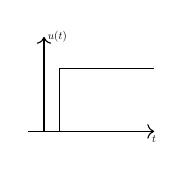
\begin{tikzpicture}[scale=0.4,every node/.style={scale=0.4}]
    % horizontal axis
    \draw[->] (0,0) -- (4,0) node[anchor=north] {$t$};
    \draw[->] (0.5,0) -- (0.5,3) node[anchor=west] {$u(t)$};
    % ranges
   \draw (1,0) -- (1,2) -- (4,2);
  \end{tikzpicture}
    \begin{circuitikz}[european,scale=0.4,every node/.style={scale=0.4}]
        \draw
        (0,0) to [short, o-] (2,0)
        to  (2,0)
        to[R] (3,0)
        to [short, -*] (4,0)
        to[C] (4,-2)
        to   (4,-2)
        (0,-2) to [short, o-*] (4,-2)
        (4,-2) to [short, -o] (7,-2)
        (4,0) to [short, -o](7,0);
     \end{circuitikz}
        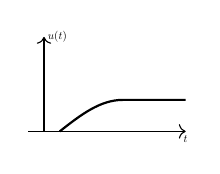
\begin{tikzpicture}[scale=0.4,every node/.style={scale=0.4}]
% horizontal axis
\draw[->] (0,0) -- (5,0) node[anchor=north] {$t$};
\draw[->] (0.5,0) -- (0.5,3) node[anchor=west] {$u(t)$};
% ranges

% Our BLock
\draw[thick] (1,0) sin (3,1) -- (5,1);

\end{tikzpicture}
  \end{center}
\end{figure}

\newpage
Besipiel 3\

\begin{figure}[h!]
  \begin{center}
    \begin{circuitikz}[european,scale=0.7,every node/.style={scale=0.7}]
        \draw
        (0,0) to [short, o-] (2,0)
        to  (2,0)
        to[C, l=$C_1$] (3,0)
        to [short, -*] (4,0)
        to[R, l=$R_1$] (4,-2)
        to   (4,-2)
        (0,-2) to [short, o-*] (4,-2)
        (4,-2) to [short, -o] (7,-2)
        (4,0) to [short, -o](7,0);
        \draw[-latex] (0,-0.1) -- (0,-1.9) node[anchor=east,midway] {$U_1$};
        \draw[-latex] (7,-0.1) -- (7,-1.9) node[anchor=west,midway] {$U_2$};;
   \end{circuitikz}
  \end{center}
\end{figure}

$ v_u(\omega) = \frac{R}{R+(\frac{1}{j \omega C})} = \frac{j \omega RC}{1 + RC \cdot \omega \cdot j} $\\
$ \omega \rightarrow 0 \leadsto v_u(\omega) = 0 $\\
$ \omega \rightarrow \infty \leadsto v_u(\omega) = 1 $\\
Grenzwert $ \omega_g = \frac{1}{RC} $\\\\
Hochpass 1. Ordnung \newline
Abtrennung oder Unterdrueckung von Gleichspannungen bezueglich Singalanteilen\\

Beispiel 4\\
\begin{figure}[h!]
  \begin{center}
    \begin{circuitikz}[european,scale=0.7,every node/.style={scale=0.7},american inductors]
        \draw
        (0,0) to [short, o-] (2,0)
        to  (2,0)
        to[L, l=$L_1$] (3,0)
        to [short, -*] (4,0)
        to[R, l=$R_1$] (4,-2)
        to   (4,-2)
        (0,-2) to [short, o-*] (4,-2)
        (4,-2) to [short, -o] (7,-2)
        (4,0) to [short, -o](7,0);
        \draw[-latex] (0,-0.1) -- (0,-1.9) node[anchor=east,midway] {$U_1$};
        \draw[-latex] (7,-0.1) -- (7,-1.9) node[anchor=west,midway] {$U_2$};;
   \end{circuitikz}
  \end{center}
\end{figure}
$ v_u(\omega) = \frac{R}{R+j\omega L} $\\
$ \left.\begin{aligned} v_u(\omega) \underset{\omega\rightarrow0}{\Bigm\vert} = 1 \\ v_u(\omega) \underset{\omega\rightarrow \infty}{\Bigm\vert} = 0  \end{aligned} \right\} \qquad \text{Tiefpass 1.Ordnung} $\\

Grenzefrequenz
 wo Real und Imaginärteil\\
 $ \leadsto R = \omega_g \cdot L $\\
 $ \omega_g = \frac{R}{L} $ \\
 $ f_g = \frac{R}{2\cdot \pi \cdot L} $\\
 Zweck: Gleichspannungsversorgung, bei welchen storend Wechslpannung unterdrueckt werden\\

\newpage
 Beispiel 5\\
 Realität "Spule hat Reihen Wderstand"
\begin{figure}[h!]
  \begin{center}
    \begin{circuitikz}[european,scale=0.7,every node/.style={scale=0.7},american inductors]
        \draw
        (0,0) to [short, o-] (1,0)
        to[L, l=$L_1$] (2,0)
        to [R, l=$R_L$] (4,0)
        to [short, -*] (5,0)
        to[R, l=$R_1$] (5,-2)
        to (5,-2)
        (4,0) to [short, -o](7,0);
        \draw [decorate,decoration={mirror,brace,amplitude=9pt},yshift=-1pt](0.5,-0.1) -- (3.6,-0.1) node [black,midway,yshift=-0.6cm] {\footnotesize Spule};
   \end{circuitikz}
  \end{center}
\end{figure}
Tiefpass 1. Ordnung\\
$ v_u(\omega) = \frac{R}{j \omega L + R_L + R} $\\
$ \omega_g = \frac{(R_L + R)}{L} $\\

Beispiel 6\\
\begin{figure}[h]
  \begin{center}
    \begin{circuitikz}[european,scale=0.7,every node/.style={scale=0.7},american inductors]
        \draw
        (0,0) to [short, o-] (1,0)
        to[L, l=$L_1$] (2,0)
        to [R, l=$R_1$] (4,0)
        to [short, -*] (5,0)
        to[L, l=$L_2$] (5,-2)
        to[R, l=$R_2$] (5,-4)
        to (5,-4)
        (5,0) to [short, -o](7,0)
        (0,-4) to [short, o-*] (5,-4)
        (5,-4) to [short, -o] (7,-4)
        (5,0) to [short, -o](7,0);
        \draw[-latex] (0,-0.1) -- (0,-3.9);
        \draw[-latex] (7,-0.1) -- (7,-3.9);
   \end{circuitikz}
  \end{center}
\end{figure}
$ v_u(\omega) = \frac{R_2 + j \omega L_2}{R_1 + R_2 + j \omega (L_1 + L_2)}= \frac{R_2 + j \omega L_2}{R_1 + j \omega + R_2 + j  \omega L_2} $\\
$ v_u(\omega) \underset{\omega\rightarrow0}{\Bigm\vert} = \frac{R_2}{R_1+R_2} \\ v_u(\omega) \underset{\omega\rightarrow \infty}{\Bigm\vert} = \frac{L_1}{L_1+L_2} $

\newpage
Beispiel 7
\begin{figure}[h]
  \begin{center}
    \begin{circuitikz}[european,scale=0.7,every node/.style={scale=0.7},american inductors]
        \draw
        (0,0) to [short, o-] (1,0)
        to[C, l=$C_1$] (2,0)
        to [L, l=$L_1$] (4,0)
        to [short, -*] (5,0)
        to[L, l=$L_2$] (5,-3)
        to (5,-4)
        (5,0) to [short, -o](7,0)
        (0,-4) to [short, o-*] (5,-4)
        (5,-4) to [short, -o] (7,-4)
        (5,0) to [short, -o](7,0);
        \draw[-latex] (0,-0.1) -- (0,-3.9);
        \draw[-latex] (7,-0.1) -- (7,-3.9);
   \end{circuitikz}
  \end{center}
\end{figure}

\input{text/15.07.2015}

% chapter _bertragungsvewrhalten_von_komplexen_schaltung_bei_sin (end)


\end{document}}
